%%%%%%%%%%%%%%%%%%%%%%%%%%%%%%%%%%%%%%%%%%%%%%%%%%%%%%%%%%%%%%%%%%%%%%%%%%%%%%%%
%%%%%%%%%%%%%%%%%%%%%%%%%%%%%%%%%%%%%%%%%%%%%%%%%%%%%%%%%%%%%%%%%%%%%%%%%%%%%%%%
\subsection{Motivation}
\label{subsec:motivation}

The proposed method's motivation lies in the simple but powerful fact that in
general is exhibited through fig. \ref{fig:motivation_caer}: Let a pose
estimate of a 2D LIDAR sensor be in a neighbourhood of its true pose within a
given map (Def. \ref{def:definition_0}); then the value of the CAER metric
(Def.  \ref{def:definition_3}) between the scan measured by the sensor (Def.
\ref{def:definition_1}) and the map-scan captured from the estimate within the
map (Def. \ref{def:definition_2}) is proportional to both the estimate's
location error and orientation error. In other words comparing any two pose
estimates residing in a neighbourhood of the sensor's pose in terms of a scalar
value is enough to establish a pose error hierarchy between them. Moreover,
this scalar locus metric is directly derivable and calculable from the
assumptions of Problem \ref{prob:the_problem}, with low computational
complexity $\mathcal{O}(N_s)$.

The relationships of proportionality between the CAER metric of a pose
estimate and its location and orientation errors have been discovered and
successfully exploited in the context of non-global localisation, and
specifically in pose-tracking, for the production of lidar odometry
\cite{Filotheou2022f} and the reduction of localisation's pose estimate error
\cite{Filotheou2023a}. In this context, estimate errors are close to the
origin, i.e. in contrast to the arbitrary distribution of hypotheses' errors in
Monte Carlo global localisation methods.


\begin{figure}\vspace{-1.5cm}
  \subfloat{\hspace{0.5cm}% GNUPLOT: LaTeX picture with Postscript
\begingroup
  \makeatletter
  \providecommand\color[2][]{%
    \GenericError{(gnuplot) \space\space\space\@spaces}{%
      Package color not loaded in conjunction with
      terminal option `colourtext'%
    }{See the gnuplot documentation for explanation.%
    }{Either use 'blacktext' in gnuplot or load the package
      color.sty in LaTeX.}%
    \renewcommand\color[2][]{}%
  }%
  \providecommand\includegraphics[2][]{%
    \GenericError{(gnuplot) \space\space\space\@spaces}{%
      Package graphicx or graphics not loaded%
    }{See the gnuplot documentation for explanation.%
    }{The gnuplot epslatex terminal needs graphicx.sty or graphics.sty.}%
    \renewcommand\includegraphics[2][]{}%
  }%
  \providecommand\rotatebox[2]{#2}%
  \@ifundefined{ifGPcolor}{%
    \newif\ifGPcolor
    \GPcolorfalse
  }{}%
  \@ifundefined{ifGPblacktext}{%
    \newif\ifGPblacktext
    \GPblacktexttrue
  }{}%
  % define a \g@addto@macro without @ in the name:
  \let\gplgaddtomacro\g@addto@macro
  % define empty templates for all commands taking text:
  \gdef\gplfronttext{}%
  \gdef\gplfronttext{}%
  \makeatother
  \ifGPblacktext
    % no textcolor at all
    \def\colorrgb#1{}%
    \def\colorgray#1{}%
  \else
    % gray or color?
    \ifGPcolor
      \def\colorrgb#1{\color[rgb]{#1}}%
      \def\colorgray#1{\color[gray]{#1}}%
      \expandafter\def\csname LTw\endcsname{\color{white}}%
      \expandafter\def\csname LTb\endcsname{\color{black}}%
      \expandafter\def\csname LTa\endcsname{\color{black}}%
      \expandafter\def\csname LT0\endcsname{\color[rgb]{1,0,0}}%
      \expandafter\def\csname LT1\endcsname{\color[rgb]{0,1,0}}%
      \expandafter\def\csname LT2\endcsname{\color[rgb]{0,0,1}}%
      \expandafter\def\csname LT3\endcsname{\color[rgb]{1,0,1}}%
      \expandafter\def\csname LT4\endcsname{\color[rgb]{0,1,1}}%
      \expandafter\def\csname LT5\endcsname{\color[rgb]{1,1,0}}%
      \expandafter\def\csname LT6\endcsname{\color[rgb]{0,0,0}}%
      \expandafter\def\csname LT7\endcsname{\color[rgb]{1,0.3,0}}%
      \expandafter\def\csname LT8\endcsname{\color[rgb]{0.5,0.5,0.5}}%
    \else
      % gray
      \def\colorrgb#1{\color{black}}%
      \def\colorgray#1{\color[gray]{#1}}%
      \expandafter\def\csname LTw\endcsname{\color{white}}%
      \expandafter\def\csname LTb\endcsname{\color{black}}%
      \expandafter\def\csname LTa\endcsname{\color{black}}%
      \expandafter\def\csname LT0\endcsname{\color{black}}%
      \expandafter\def\csname LT1\endcsname{\color{black}}%
      \expandafter\def\csname LT2\endcsname{\color{black}}%
      \expandafter\def\csname LT3\endcsname{\color{black}}%
      \expandafter\def\csname LT4\endcsname{\color{black}}%
      \expandafter\def\csname LT5\endcsname{\color{black}}%
      \expandafter\def\csname LT6\endcsname{\color{black}}%
      \expandafter\def\csname LT7\endcsname{\color{black}}%
      \expandafter\def\csname LT8\endcsname{\color{black}}%
    \fi
  \fi
  \setlength{\unitlength}{0.0500bp}%
  \begin{picture}(6000.00,4000.00)%
    \gplgaddtomacro\gplfronttext{%
      \colorrgb{0.00,0.00,0.00}%
      \colorrgb{0.00,0.00,0.00}%
      \put(445,1460){\makebox(0,0)[r]{\strut{}\scriptsize $-\pi$}}%
      \colorrgb{0.00,0.00,0.00}%
      \put(822,1360){\makebox(0,0)[r]{\strut{}\scriptsize $-\pi/2$}}%
      \colorrgb{0.00,0.00,0.00}%
      \colorrgb{0.00,0.00,0.00}%
      \put(1199,1260){\makebox(0,0)[r]{\strut{}\scriptsize $0.0$}}%
      \colorrgb{0.00,0.00,0.00}%
      \colorrgb{0.00,0.00,0.00}%
      \put(1577,1160){\makebox(0,0)[r]{\strut{}\scriptsize $+\pi/2$}}%
      \colorrgb{0.00,0.00,0.00}%
      \put(1954,1060){\makebox(0,0)[r]{\strut{}\scriptsize $+\pi$}}%
      \colorrgb{0.00,0.00,0.00}%
      \colorrgb{0.00,0.00,0.00}%
      \put(2444,979){\makebox(0,0){\strut{}\scriptsize $0.0$}}%
      \colorrgb{0.00,0.00,0.00}%
      \put(3042,1057){\makebox(0,0){\strut{}\scriptsize $10.0$}}%
      \colorrgb{0.00,0.00,0.00}%
      \put(3642,1135){\makebox(0,0){\strut{}\scriptsize $20.0$}}%
      \colorrgb{0.00,0.00,0.00}%
      \put(4241,1213){\makebox(0,0){\strut{}\scriptsize $30.0$}}%
      \colorrgb{0.00,0.00,0.00}%
      \put(594,1526){\makebox(0,0)[r]{\strut{}\scriptsize $0$}}%
      \colorrgb{0.00,0.00,0.00}%
      \put(594,1869){\makebox(0,0)[r]{\strut{}\scriptsize $400$}}%
      \colorrgb{0.00,0.00,0.00}%
      \put(594,2212){\makebox(0,0)[r]{\strut{}\scriptsize $800$}}%
      \colorrgb{0.00,0.00,0.00}%
      \put(594,2555){\makebox(0,0)[r]{\strut{}\scriptsize $1200$}}%
      \colorrgb{0.00,0.00,0.00}%
      %\put(-115,2129){\rotatebox{90}{\makebox(0,0){\strut{}\scriptsize CAER [m]}}}%
      \colorrgb{0.00,0.00,0.00}%
      %\put(2640,2854){\makebox(0,0){\strut{}title}}%
    }%
    \gplgaddtomacro\gplfronttext{%
      \colorrgb{0.00,0.00,0.00}%
      \put(679,1037){\rotatebox{-22}{\makebox(0,0){\strut{}\footnotesize Orientation error $\Delta\hat{\theta}$ [rad]}}}%
      \colorrgb{0.00,0.00,0.00}%
      \put(3621,852){\rotatebox{7}{\makebox(0,0){\strut{}\footnotesize Position error $\|\Delta\hat{\bm{l}}\|_2$ [m]}}}%
      \colorrgb{0.00,0.00,0.00}%
      \put(-115,2129){\rotatebox{90}{\makebox(0,0){\strut{}\footnotesize CAER [m]}}}%
    }%
    \gplgaddtomacro\gplfronttext{%
    }%
    \gplgaddtomacro\gplfronttext{%
      \colorrgb{0.00,0.00,0.00}%
%      \put(5375,1039){\makebox(0,0)[l]{\strut{}\scriptsize $0$}}%
      %\colorrgb{0.00,0.00,0.00}%
      %\put(5375,1624){\makebox(0,0)[l]{\strut{}\scriptsize $400$}}%
      %\colorrgb{0.00,0.00,0.00}%
      %\put(5375,2209){\makebox(0,0)[l]{\strut{}\scriptsize $800$}}%
      %\colorrgb{0.00,0.00,0.00}%
      %\put(5375,2795){\makebox(0,0)[l]{\strut{}\scriptsize $1200$}}%
      %\colorrgb{0.00,0.00,0.00}%
      %\put(5375,3087){\makebox(0,0)[l]{\strut{}\scriptsize $1400$}}%
    }%
    \put(0,0){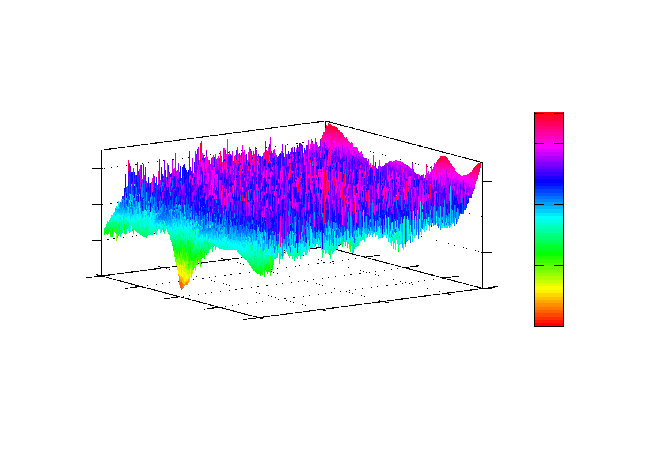
\includegraphics[trim={0 0 2cm 1.4cm},clip]{./figures/caer_all}}%
    \gplfronttext
  \end{picture}%
\endgroup
}\vspace{-1.5cm}\\
  \subfloat{\hspace{-0.3cm}% GNUPLOT: LaTeX picture with Postscript
\begingroup
  \makeatletter
  \providecommand\color[2][]{%
    \GenericError{(gnuplot) \space\space\space\@spaces}{%
      Package color not loaded in conjunction with
      terminal option `colourtext'%
    }{See the gnuplot documentation for explanation.%
    }{Either use 'blacktext' in gnuplot or load the package
      color.sty in LaTeX.}%
    \renewcommand\color[2][]{}%
  }%
  \providecommand\includegraphics[2][]{%
    \GenericError{(gnuplot) \space\space\space\@spaces}{%
      Package graphicx or graphics not loaded%
    }{See the gnuplot documentation for explanation.%
    }{The gnuplot epslatex terminal needs graphicx.sty or graphics.sty.}%
    \renewcommand\includegraphics[2][]{}%
  }%
  \providecommand\rotatebox[2]{#2}%
  \@ifundefined{ifGPcolor}{%
    \newif\ifGPcolor
    \GPcolorfalse
  }{}%
  \@ifundefined{ifGPblacktext}{%
    \newif\ifGPblacktext
    \GPblacktexttrue
  }{}%
  % define a \g@addto@macro without @ in the name:
  \let\gplgaddtomacro\g@addto@macro
  % define empty templates for all commands taking text:
  \gdef\gplfronttext{}%
  \gdef\gplfronttext{}%
  \makeatother
  \ifGPblacktext
    % no textcolor at all
    \def\colorrgb#1{}%
    \def\colorgray#1{}%
  \else
    % gray or color?
    \ifGPcolor
      \def\colorrgb#1{\color[rgb]{#1}}%
      \def\colorgray#1{\color[gray]{#1}}%
      \expandafter\def\csname LTw\endcsname{\color{white}}%
      \expandafter\def\csname LTb\endcsname{\color{black}}%
      \expandafter\def\csname LTa\endcsname{\color{black}}%
      \expandafter\def\csname LT0\endcsname{\color[rgb]{1,0,0}}%
      \expandafter\def\csname LT1\endcsname{\color[rgb]{0,1,0}}%
      \expandafter\def\csname LT2\endcsname{\color[rgb]{0,0,1}}%
      \expandafter\def\csname LT3\endcsname{\color[rgb]{1,0,1}}%
      \expandafter\def\csname LT4\endcsname{\color[rgb]{0,1,1}}%
      \expandafter\def\csname LT5\endcsname{\color[rgb]{1,1,0}}%
      \expandafter\def\csname LT6\endcsname{\color[rgb]{0,0,0}}%
      \expandafter\def\csname LT7\endcsname{\color[rgb]{1,0.3,0}}%
      \expandafter\def\csname LT8\endcsname{\color[rgb]{0.5,0.5,0.5}}%
    \else
      % gray
      \def\colorrgb#1{\color{black}}%
      \def\colorgray#1{\color[gray]{#1}}%
      \expandafter\def\csname LTw\endcsname{\color{white}}%
      \expandafter\def\csname LTb\endcsname{\color{black}}%
      \expandafter\def\csname LTa\endcsname{\color{black}}%
      \expandafter\def\csname LT0\endcsname{\color{black}}%
      \expandafter\def\csname LT1\endcsname{\color{black}}%
      \expandafter\def\csname LT2\endcsname{\color{black}}%
      \expandafter\def\csname LT3\endcsname{\color{black}}%
      \expandafter\def\csname LT4\endcsname{\color{black}}%
      \expandafter\def\csname LT5\endcsname{\color{black}}%
      \expandafter\def\csname LT6\endcsname{\color{black}}%
      \expandafter\def\csname LT7\endcsname{\color{black}}%
      \expandafter\def\csname LT8\endcsname{\color{black}}%
    \fi
  \fi
    \setlength{\unitlength}{0.0500bp}%
    \ifx\gptboxheight\undefined%
      \newlength{\gptboxheight}%
      \newlength{\gptboxwidth}%
      \newsavebox{\gptboxtext}%
    \fi%
    \setlength{\fboxrule}{0.5pt}%
    \setlength{\fboxsep}{1pt}%
\begin{picture}(5000.00,3000.00)%
    \gplgaddtomacro\gplfronttext{%
    }%
    \gplgaddtomacro\gplfronttext{%
      \colorrgb{0.15,0.15,0.15}%
      \put(336,1498){\makebox(0,0)[r]{\strut{}}}%
      \colorrgb{0.15,0.15,0.15}%
      \put(336,1905){\makebox(0,0)[r]{\strut{}}}%
      \colorrgb{0.15,0.15,0.15}%
      \put(336,2312){\makebox(0,0)[r]{\strut{}}}%
      \colorrgb{0.15,0.15,0.15}%
      \put(300,1905){\rotatebox{90}{\makebox(0,0){\strut{}$\Delta\hat{\theta} \in [-\pi,\pi)$ rad}}}%
      %\put(400,933){\makebox(0,0){\strut{}\small $0.0$}}%
      \colorrgb{0.15,0.15,0.15}%
      \put(871,933){\makebox(0,0){\strut{}\small $0.5$}}%
      \colorrgb{0.15,0.15,0.15}%
      \put(1342,933){\makebox(0,0){\strut{}\small $1.0$}}%
      \colorrgb{0.15,0.15,0.15}%
      \put(1813,933){\makebox(0,0){\strut{}\small $1.5$}}%
      \colorrgb{0.15,0.15,0.15}%
      \put(2285,933){\makebox(0,0){\strut{}\small $2.0$}}%
      \colorrgb{0.15,0.15,0.15}%
      \put(1487,663){\makebox(0,0){\strut{}$\|\Delta \hat{\bm{l}}\|_2$ [m]}}%
    }%
    \gplgaddtomacro\gplfronttext{%
    }%
    \gplgaddtomacro\gplfronttext{%
      \colorrgb{0.15,0.15,0.15}%
      \put(5113,1110){\makebox(0,0)[l]{\strut{}}}%
      \colorrgb{0.15,0.15,0.15}%
      \put(5113,1110){\makebox(0,0)[l]{\strut{}}}%
      \colorrgb{0.15,0.15,0.15}%
      \put(5113,1110){\makebox(0,0)[l]{\strut{}}}%
      %\put(2875,933){\makebox(0,0){\strut{}\small $0.0$}}%
      \colorrgb{0.15,0.15,0.15}%
      \put(3346,933){\makebox(0,0){\strut{}\small $0.5$}}%
      \colorrgb{0.15,0.15,0.15}%
      \put(3817,933){\makebox(0,0){\strut{}\small $1.0$}}%
      \colorrgb{0.15,0.15,0.15}%
      \put(4288,933){\makebox(0,0){\strut{}\small $1.5$}}%
      \colorrgb{0.15,0.15,0.15}%
      \put(4760,933){\makebox(0,0){\strut{}\small $2.0$}}%
      \colorrgb{0.15,0.15,0.15}%
      \put(2762,1905){\rotatebox{90}{\makebox(0,0){\strut{}\small CAER [m]}}}
      \put(3987,663){\makebox(0,0){\strut{}$\|\Delta \hat{\bm{l}}\|_2$ [m]}}%
    }%
    \gplgaddtomacro\gplfronttext{%
    }%
    \gplgaddtomacro\gplfronttext{%
    }%
    \gplgaddtomacro\gplfronttext{%
    }%
    \gplgaddtomacro\gplfronttext{%
      \put(500,80){\makebox(0,0){\strut{}$\footnotesize 0$}}%
      \colorrgb{0.15,0.15,0.15}%
%      \put(1390,80){\makebox(0,0){\strut{}$\footnotesize 60$}}%
      %\colorrgb{0.15,0.15,0.15}%
      %\put(2280,80){\makebox(0,0){\strut{}$\footnotesize 270$}}%
      %\colorrgb{0.15,0.15,0.15}%
      %\put(3169,80){\makebox(0,0){\strut{}$\footnotesize 540$}}%
      %\colorrgb{0.15,0.15,0.15}%
      %\put(4059,80){\makebox(0,0){\strut{}$\footnotesize 810$}}%
      \colorrgb{0.15,0.15,0.15}%
      \put(4849,80){\makebox(0,0){\strut{}$\footnotesize 1080$}}%
    }%
    \put(0,0){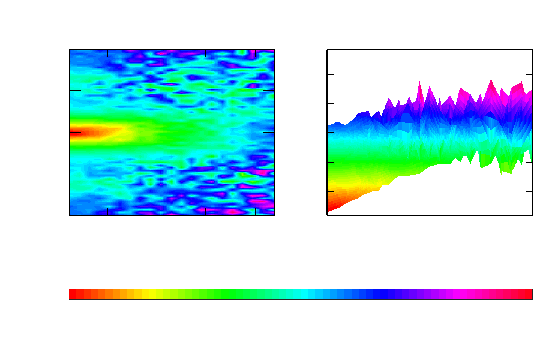
\includegraphics{./figures/face_bottom}}%
    \gplfronttext
  \end{picture}%
\endgroup
}
  \caption{\small Top: without loss o generality, a typical plot of the
           Cumulative Absolute Error per Ray metric (Eq. (\ref{eq:caer})) of
           $10^6$ hypotheses disperesed in the map of environment WAREHOUSE
           (Fig. \ref{fig:face} and section \ref{subsec:exp_b}). Bottom:
           focused view on hypotheses with location error close to the origin}
  \vspace{-0.5cm}
  \label{fig:motivation_caer}
\end{figure}


The above motivate investigation on whether the CAER metric could prove equally
beneficial in settings more uncertain than pose-tracking, that is, where the
location and orientation of pose estimates extend farther away from the
sensor's true location and orientation. Fig. \ref{fig:h_and_h_not_fig} (top)
shows the relations between the total errors of hypotheses and
their (a) CAER values (left) and (b) resulting ranks (right),
which resulted from an experimental procedure similar to that which produced fig.
\ref{fig:motivation_caer}.

%%%%%%%%%%%%%%%%%%%%%%%%%%%%%%%%%%%%%%%%%%%%%%%%%%%%%%%%%%%%%%%%%%%%%%%%%%%%%%%%
%%%%%%%%%%%%%%%%%%%%%%%%%%%%%%%%%%%%%%%%%%%%%%%%%%%%%%%%%%%%%%%%%%%%%%%%%%%%%%%%
\subsection{The CBGL System}

In order to test the efficacy of the CAER metric in aiding the solution of
Problem \ref{prob:the_problem}, we introduce the CAER-Based Global Localisation
system (CBGL).\footnote{For a rigorous mathematical formulation of the
hypothesis underpinning CBGL see \cite{cbglarxiv}.} Given map $\bm{M}$, CBGL
first generates a set of pose hypotheses $\mathcal{H}$ (Def.
\ref{def:definition_0}). Their positions are randomly generated
uniformly within the map's traversable space, while orientations within
$[-\pi,\pi)$ rad. Then from these poses it computes map-scans (Def.
\ref{def:definition_2}). Given these map-scans and a LIDAR's 2D measurement
$\mathcal{S}_R$ (Def. \ref{def:definition_1}), CBGL subsequently computes the
CAER value (Def. \ref{def:definition_3}) associated with each pose hypothesis.
It then ranks them in ascending order and selects the $k$ estimates with the
least CAER values in an attempt to estimate the $k$ hypotheses with the least
pose error (Alg. \ref{alg:bottom_k}). Estimation in this sense rests on the
motivation of subsection \ref{subsec:motivation}.

One challenge is choosing such $k$, $d_{\bm{l}}$, and $d_\alpha$ (Def.
\ref{def:definition_6}) that, given pose estimate error requirements
$\delta_{\bm{l}}$, $\delta_{\theta}$, CBGL produces admissible pose estimates
(Def. \ref{def:definition_7}) while being executed in timely manner.  Given the
rank field's Monte Carlo nature, optimistically, the only option for increasing
the accuracy of the final pose estimate by a factor of two would be to double
the densities of the \texttt{r}-field; instead of doing that---and thereby
doubling the method's execution time---subsequent to the estimation of the pose
estimates with the $k$ lowest CAER values, CBGL utilises scan--to--map-scan
matching \cite{Vasiljevic2016c,Filotheou2023a}, followed by the estimation of
the one pose estimate with the lowest CAER value within the group of $k$
matched estimates.

Matching allows for (a) the correction of the pose of true positive estimates
by scan-matching the map-scan captured from a pose estimate against the range
scan measured by the real sensor, (b) by the same token the potential
divergence of spurious, false positive, pose estimates, and hence their
elimination as pose estimate candidates, (c) the production of finer pose
estimates without excessive increase in execution time, and (d) the decoupling
of the final pose estimate's error from the field's densities.

CBGL's output pose estimate is that with the least CAER among the $k$ matched
estimates. CBGL is described in block diagram form in figure
\ref{fig:block_system} (left) and in pseudocode in Algorithm \ref{alg:cbgl}.


\begin{figure}\vspace{-0.4cm}
  \subfloat{\label{fig:cbgl}     \input{./figures/cbgl_system_tiny.tikz}}
  \subfloat{\label{fig:bottom_k} \input{./figures/inner_ranking_system2_tiny.tikz}}
  \caption{\small CBGL in block diagram form. Left: Given map $\bm{M}$, CBGL
           first generates a set of pose hypotheses $\mathcal{H}$. Then it
           estimates the $k$ hypotheses with the least pose error (right; Alg.
           \ref{alg:bottom_k}).
           %II \cite{Filotheou2023c}
           As a final step, it scan--to--map-scan
           matches these to $\mathcal{S}_R$ for finer estimation
           (\texttt{sm2}; Alg.
           \ref{alg:sm2}).
           %III \cite{Filotheou2023c}
           CBGL's output pose estimate is that with
           the minimum CAER among the $k$ matched estimates
           }
\vspace{-0.5cm}
  \label{fig:block_system}
\end{figure}


%%% CBGL %%%%%%%%%%%%%%%%%%%%%%%%%%%%%%%%%%%%%%%%%%%%%%%%%%%%%%%%%%%%%%%%%%%%%%%%
\begin{algorithm}[]
  \caption{\texttt{CBGL}}
  \begin{spacing}{1.0}
  \begin{algorithmic}[1]
    \REQUIRE $\mathcal{S}_R$, $\lambda$, $\bm{M}$, $(d_{\bm{l}}, d_\alpha)$, $k$
    \ENSURE Pose estimate of sensor measuring range scan $\mathcal{S}_R$ %$\hat{\bm{p}}$
    \STATE $A \leftarrow \texttt{calculate\_area}(\texttt{free}(\bm{M}))$
    \STATE $\mathcal{H} \leftarrow \{\varnothing\}$
    \FOR {$i \leftarrow 0,1,\dots,d_{\bm{l}} \cdot A-1$}
      \STATE \small $(\hat{x},\hat{y},\hat{\theta}) \leftarrow \texttt{rand()}$: $(x,y) \in \texttt{free}(\bm{M})$, $\hat{\theta} \in [-\pi,+\pi)$
      \FOR {$j \leftarrow 0,1,\dots, d_{\alpha}-1$}
        \STATE $\mathcal{H} \leftarrow \{\mathcal{H}, (\hat{x}, \hat{y}, \hat{\theta} + j \cdot 2\pi / d_{\alpha})\}$     \label{alg:cbgl:h}
      \ENDFOR
    \ENDFOR
    \STATE $\mathcal{H}_1 \leftarrow$ \texttt{bottom}$\_k\_\texttt{poses}(\mathcal{S}_R, \bm{M}, \mathcal{H}, k)$ \hfill {\small (Alg. \ref{alg:bottom_k}}) \label{alg:cbgl:h1}
    \STATE $\mathcal{H}_2 \leftarrow \{\varnothing \}$
    \FOR {$k \leftarrow 0,1,\dots,|\mathcal{H}_1|-1$}
      \STATE $\hat{\bm{h}}^\prime \leftarrow \texttt{sm2}(\mathcal{S}_R, \lambda, \bm{M}, \mathcal{H}_1[k])$ \hfill {\small (Alg. \ref{alg:sm2}---e.g. \texttt{x1} \cite{Filotheou2023a}})
      \STATE $\mathcal{H}_2 \leftarrow \{\mathcal{H}_2, \hat{\bm{h}}^\prime\}$  \label{alg:cbgl:h2}
    \ENDFOR
    \RETURN \texttt{bottom}$\_k\_\texttt{poses}(\mathcal{S}_R, \bm{M}, \mathcal{H}_2, 1)$
  \end{algorithmic}
  \end{spacing}
  \label{alg:cbgl}
\end{algorithm}

%% Bottom-n %%%%%%%%%%%%%%%%%%%%%%%%%%%%%%%%%%%%%%%%%%%%%%%%%%%%%%%%%%%%%%%%%%%%
\begin{algorithm}[]
  \caption{\texttt{bottom}\_$k$\_\texttt{poses}}
  \begin{spacing}{1.0}
  \begin{algorithmic}[1]
    \REQUIRE $\mathcal{S}_R$, $\bm{M}$, $\mathcal{H}$, $k$
    \ENSURE Set of $k$ poses of $\mathcal{H}$ with least CAER values, $\mathcal{H}_{\triangledown}$
    \STATE $\Psi \leftarrow \{\varnothing \}$
    \FOR {$h \leftarrow 0,1,\dots,|\mathcal{H}|-1$}
      \STATE $\mathcal{S}_V^{\hspace{1pt} h} \leftarrow \texttt{scan\_map}(\bm{M}, \mathcal{H}[h])$
      \STATE $\psi \leftarrow 0$
      \FOR {$n \leftarrow 0,1,\dots,|\mathcal{S}_R|-1$}
        \STATE $\psi \leftarrow \psi + \big|\mathcal{S}_R[n]-\mathcal{S}_V^{\hspace{1pt} h}[n]\big|$ \hfill {\small (Eq. (\ref{eq:caer})})
      \ENDFOR
      \STATE $\Psi \leftarrow \{\Psi, \psi\}$
    \ENDFOR
    \STATE $[\Psi_{\uparrow}, \texttt{I}^{\ast}] \leftarrow \texttt{sort}(\Psi, \texttt{asc})$
    \STATE $\mathcal{H}_{\triangledown} \leftarrow \{\varnothing \}$
    \FOR {$h \leftarrow 0,1,\dots,k-1$}
      \STATE $\mathcal{H}_{\triangledown} \leftarrow \{\mathcal{H}_{\triangledown}, \mathcal{H}[\texttt{I}^{\ast}[h]]\}$
    \ENDFOR
    \RETURN $\mathcal{H}_{\triangledown}$
  \end{algorithmic}
  \end{spacing}
  \label{alg:bottom_k}
\end{algorithm}

%% sm2 %%%%%%%%%%%%%%%%%%%%%%%%%%%%%%%%%%%%%%%%%%%%%%%%%%%%%%%%%%%%%%%%%%%%%%%%%
\begin{algorithm}[]
  \caption{\texttt{sm2}}
  \begin{spacing}{1.0}
  \begin{algorithmic}[1]
    \REQUIRE $\mathcal{S}_R$, $\lambda$, $\bm{M}$, $\hat{\bm{p}}$
    %\ENSURE $\hat{\bm{p}}^\prime$
    \ENSURE $\hat{\bm{p}}$ $+$ correction that aligns $\mathcal{S}_V^{\bm{M}}(\hat{\bm{p}})$ to $\mathcal{S}_R$
    \STATE $\mathcal{S}_V \leftarrow \texttt{scan\_map}(\bm{M}, \hat{\bm{p}}, \lambda)$
    \STATE $\bm{\Delta p} \leftarrow \texttt{scan-match}(\mathcal{S}_R,\mathcal{S}_V)$ \hfill {\small (e.g. \texttt{ICP}\cite{Vizzo2023}, \texttt{FSM}\cite{Filotheou2022f}})
    %\STATE $\hat{\bm{p}}^\prime \leftarrow \hat{\bm{p}} + \bm{\Delta p}$
    %\RETURN $\hat{\bm{p}}^\prime$
    \RETURN $\hat{\bm{p}} + \bm{\Delta p}$
  \end{algorithmic}
  \end{spacing}
  \label{alg:sm2}
\end{algorithm}
